\documentclass[12pt,a4paper]{book}
\usepackage[utf8]{inputenc}
\usepackage{amsmath}
\usepackage{amsfonts}
\usepackage{amssymb}
\usepackage{CJKutf8}

%%%%
%设置页边距
\usepackage{geometry}
\geometry{left=1cm,right=1cm,top=1.5cm,bottom=1.5cm}
\usepackage{xcolor}
\usepackage{graphicx}
\usepackage{indentfirst} 
\usepackage{ulem}
\usepackage{tikz}	% 绘图
\usepackage{framed} % 加边框
\usepackage[colorlinks,linkcolor=black,citecolor=green]{hyperref}  % 超链接
\usepackage{bm}  % 公式粗体
\usepackage{makecell} %表格项多行


\includeonly{chp/Math,
chp/BackPropagation,
%chp/NetWorks,
chp/Whiten,
chp/Transfer_Learning}
%%%%%%%%%%%%%%%%%%%%%%%%%%%%%%%%%%%%%%%%%%%%%%%%
\begin{document}
\begin{CJK}{UTF8}{gkai}

%% 目录  %%%%%%%%%%%%%%%%%%%%%%%%%%%%%%%%%%%%%%%%
\tableofcontents
\chapter{Math}

\section{定义}
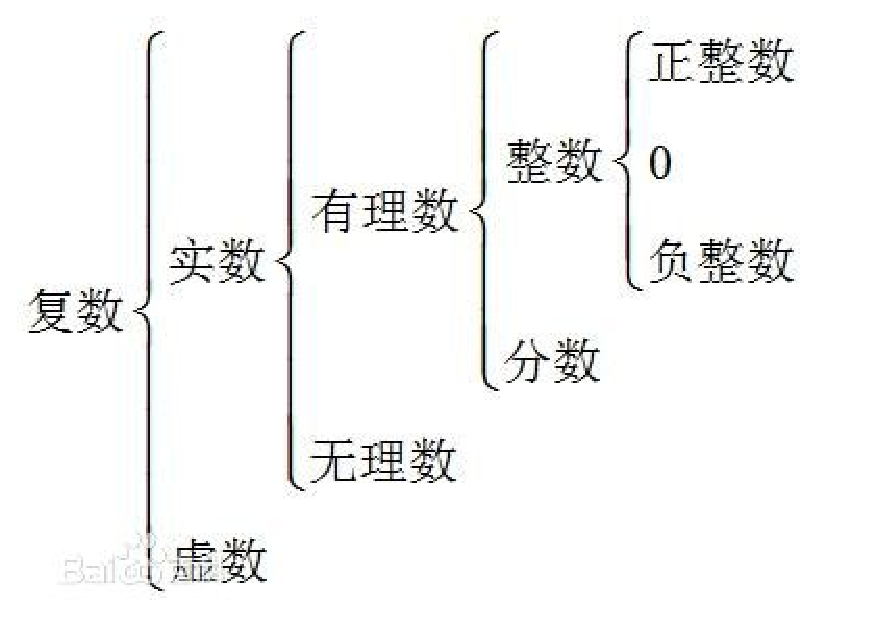
\includegraphics[scale=0.4]{fig/numbers.eps}
\cite{_infimum_????}\par
infimum——下确界,缩写 inf,复数 infima \par
supremum——上确界,缩写 sup,复数 suprema

\subsection{柯西序列(Cauchy sequence)}
\cite{_cauchy_????}
is a sequence whose elements become arbitrarily close to each other as the sequence progresses. More precisely, given any small positive distance, all but a finite number of elements of the sequence are less than that given distance from each other.\par
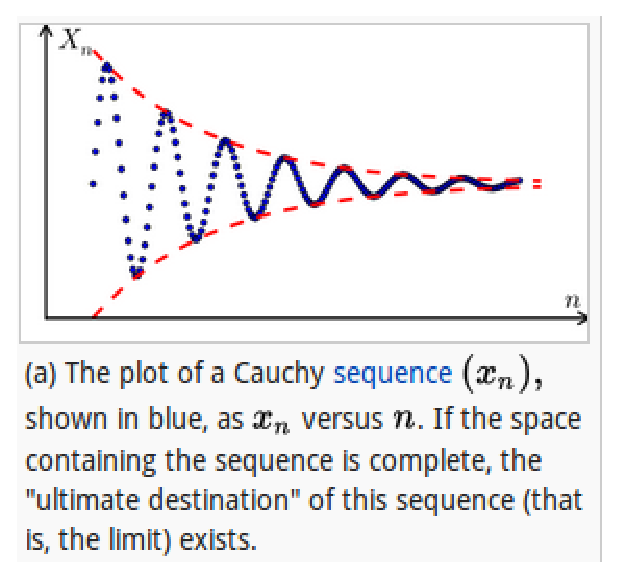
\includegraphics[scale=0.5]{fig/Cauchy_exam.eps}
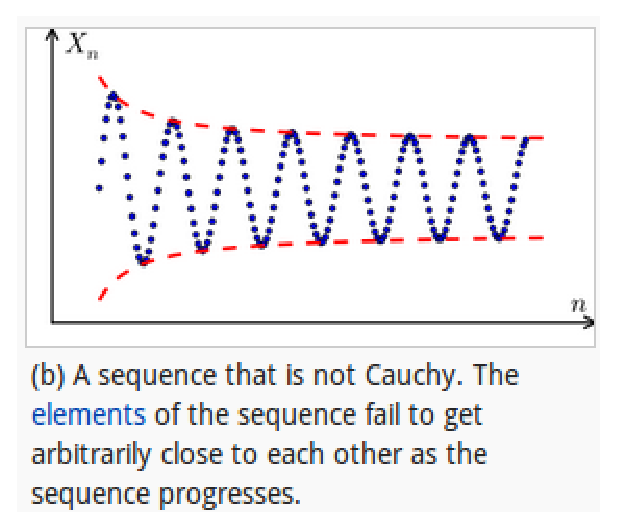
\includegraphics[scale=0.5]{fig/Cauchy_not.eps}

\subsection{完备(Completeness)(\underline{by mg:柯西序列收敛与此})}
\cite{_cauchy_????}
A metric space $X$ in which every Cauchy sequence converges to an element of $X$ is called \textbf{complete}.

\subsection{紧空间(Compact spaces)(\underline{by mg:都有子序列收敛于此})}
\cite{_cauchy_????}
A metric space $M$ is \textbf{compact} if every sequence in $M$ \underline{has a} subsequence that converges to a point in $M$. This is known as sequential compactness and, in metric spaces (but not in general topological spaces), is equivalent to the topological notions of countable compactness and compactness defined via open covers.

\subsection{赫米特矩阵 (Hermitian matrix)}
共轭转置(conjugate transpose)等于自身的矩阵(主要针对复数情况):
\[ a_{ij}= \overline{a_{ji}} \ \text{或者} \  A=\overline{A^T}\]
可以认为是对实对称矩阵的扩展。

\subsection{格拉姆矩阵 (Gramian matrix)}
In linear algebra, the Gram matrix (Gramian matrix or Gramian) of a set of vectors $v_1, \dots, v_n$ in an inner product space is the Hermitian matrix of \textbf{inner products}, whose entries are given by $G_{ij}=\left< v_i,v_j \right>$






\subsection{正定}
\subsubsection{正定函数 }

\subsubsection{正定矩阵 positive definite matrix} 
\cite{_positive-definite_????}
In linear algebra, a symmetric $n \times n$ real matrix $M$ is said to be \textbf{positive definite} if the scalar $z^T M z$ is positive for every non-zero column vector $z$ of $n$ real numbers.

例如,$I=\begin{bmatrix} 1 & 0 \\ 0 & 1\end{bmatrix}$ 是正定的。Seen as a real matrix, it is symmetric, and, for any non-zero column vector z with real entries a and b, one has
\[ z^TIz=[a \ b] \begin{bmatrix} 1 & 0 \\ 0 & 1\end{bmatrix} \begin{bmatrix} a \\ b\end{bmatrix} =a^2+b^2 \]



\section{拓扑}
\subsection{Topology(by mg:重点在连续)}
\cite{_topology_????}

\textbf{topology} is concerned with the properties of space that are preserved under \textbf{continuous deformations}, such as stretching and bending, but not tearing or gluing. This can be studied by considering a collection of subsets, called open sets, that satisfy certain properties, turning the given set into what is known as a topological space. Important topological properties include connectedness and compactness.

Formally, let $X$ be a set and let $\tau$ be a family of subsets of $X$. Then $\tau$ is called a topology on $X$ if:\par
1. Both the empty set and $X$ are elements of $\tau$ \par
2. Any union of elements of $\tau$ is an element of $\tau$ \par
3. Any intersection of finitely many elements of $\tau$ is an element of $\tau$\par
If $\tau$ is a topology on $X$, then the pair $(X, \tau)$ is called a \textbf{topological space}. The notation $X_\tau$ may be used to denote a set $X$ endowed with the particular topology $\tau$.

\subsection{Topological vector space}
\cite{_topological_????}

A topological vector space $X$ is a vector space over a topological field $K$ (most often the real or complex numbers with their standard topologies) that is endowed with a topology such that vector addition $X \times X \rightarrow X$ and scalar multiplication $K \times X \rightarrow X$ are \textbf{continuous functions }(where the domains of these functions are endowed with product topologies).

\section{度量}
\subsection{Metric space(\underline{by mg: 定义了距离})}
\cite{_metric_????}

A metric space is a set for which distances between all members of the set are defined. Those distances, taken together, are called a \textbf{metric} on the set.\par
正式定义:A metric space is an ordered pair $(M,d)$ where $M$ is a set and $d$ is a metric on $M$, i.e., a function, $d: M \times M \rightarrow R$ , such that for any $x, y, z \in M$  , the following holds:\par
\begin{tabular}[l]{lll}
\hline
1. & $d(x,y) \geq 0$ & non-negativity or separation axiom \\ 
2. & $d(x,y)=0 \Leftrightarrow x=y$ & Identity of Indiscernibles \\ 
3. & $d(x,y)=d(y,x)$ & symmetry \\ 
4. & $d(x,z) \leq d(x,y) + d(y,z)$ & subadditivity or trangle inequality\\
\hline
\end{tabular}

\subsection{完备(度量)空间(Complete metric space)(\underline{by mg: 柯西序列收敛于此})}
\cite{_complete_????}
A metric space $M$ is called complete (or a Cauchy space) if every \textbf{Cauchy sequence }of points in $M$ has a limit that is also in $M$ or, alternatively, if every Cauchy sequence in $M$ converges in $M$.\par
Intuitively, a space is complete if there are no "points missing" from it (inside or at the boundary). For instance, the set of rational numbers is not complete, because e.g. $\sqrt 2$ is "missing" from it, even though one can construct a Cauchy sequence of rational numbers that converges to it. It is always possible to "fill all the holes", leading to the completion of a given space.


\section{范函}

\subsection{范数 (Norm)(\underline{by mg:向量的量化})}
\cite{_norm_????}
A norm is a function that assigns a strictly positive length or size to each vector in a vector space—save for the zero vector, which is assigned a length of zero. A \textbf{seminorm}, on the other hand, is allowed to assign zero length to some non-zero vectors (in addition to the zero vector).\par
Given a vector space $V$ over a subfield $F$ of the complex numbers, a norm on $V$ is a function $p: V \rightarrow R$ with the following properties:\par
For all $a\in F$ and all $u, v \in V$,\par
1. $p(a\bm v) = |a| p(\bm v)$, (absolute homogeneity or absolute scalability).\par
2. $p(\bm u + \bm v) \leq p(\bm u) + p(\bm v)$ (triangle inequality or subadditivity).\par
3. If $p(\bm v) = 0$ then $\bm v$ is the zero vector (separates points).
例:\par
\begin{itemize}
\item{Absolute-value norm : $\|x\|=|x|$} 
\item{Euclidean norm ($L^2$ norm) : $ \|x\| : \sqrt{x_1^2+\dots+x_n^2}$ }
\item{Taxicab norm or Manhattan norm ($l_1$ norm): $\|x\|_1 := \sum_{i=1}^n |x_i|$}
\item{p-norm : $\|x\|_p := \left( \sum_{i=1}^n |x_i|^p \right) ^\frac{1}{p}$ }\par
The partial derivative of the p-norm \par
\[ \frac{\partial}{\partial x_k} \|x\|_p = \frac{x_k |x_k|^{p-2}}{\|x_k\|_p^{p-1}} \]
The derivative with respect to x \par
\[ \frac{\partial \|x\|_p}{\partial x} = \frac{x \circ |x_k|^{p-2}}{\|x\|_p^{p-1}} \]
where $\circ$ denotes Hadamard product and $|\cdot|$ is used for absolute value of each component of the vector.
\item{Maximum norm (special case of: infinity norm, uniform norm, or supremum norm)}
If $\bm x=(x_1,x_2,\dots,x_n)$,then:\par
\[ \|x\|_\infty := max(|x_1|,\dots,|x_n|) \]
\end{itemize}


The concept of \textbf{unit circle} (the set of all vectors of norm 1) is different in different norms: for the 1-norm the unit circle in $R^2$ is a square, for the 2-norm (Euclidean norm) it is the well-known unit circle, while for the infinity norm it is a different square. For any p-norm it is a superellipse (with congruent axes).\par
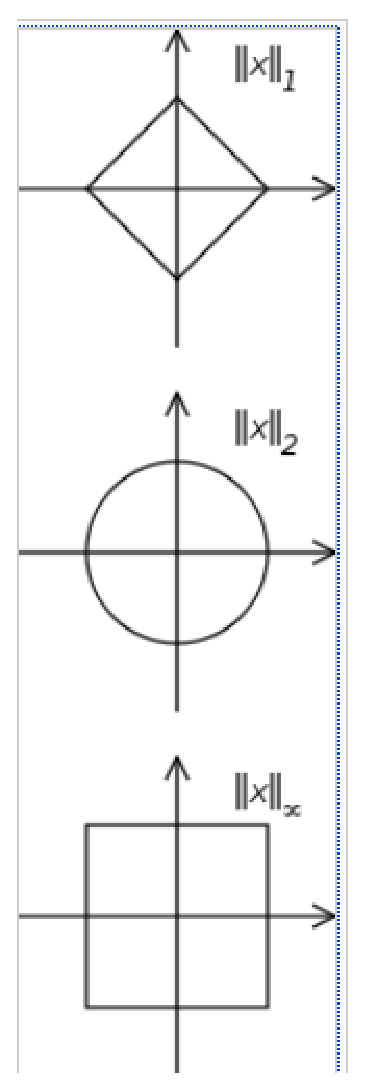
\includegraphics[scale=0.5]{fig/exp_norm_unit_circle.eps}

\subsection{向量空间 (vector space)}
\cite{_vector_????}
A vector space (also called a \textbf{linear space}) is a collection of objects called \textbf{vectors}, which may be added together and multiplied ("scaled") by numbers, called \textbf{scalars} in this context. \par
A vector space over a field $F$ is a set $V$ together with two operations that satisfy the eight axioms listed below. Elements of $V$ are commonly called \textbf{vectors}. Elements of $F$ are commonly called \textbf{scalars}. \par

\begin{tabular}[l]{|l|l|l|}
\hline
1 & Associativity of addition(结合律) & $\bm u + (\bm v + \bm w) = (\bm u + \bm v) + \bm w$ \\ \hline
2 & Commutativity of addition(交换律) & $\bm u + \bm v = \bm v + \bm u$ \\ \hline
3 & Identity element of addition & \makecell[l]{There exists an element $0 \in V$, \\ called the \textbf{zero vector}, \\such that $\bm v + 0 = \bm v$ for all $ v \in V$.} \\ \hline
4 & Inverse elements of addition & \makecell[l]{For every $ \bm v \in V$, \\there exists an element $ \textnormal{-} \bm v \in V$,\\ called the \textbf{additive inverse} of $ \bm v$, \\such that $\bm v + (\textnormal{-}\bm v) = 0$.} \\ \hline
5 & \makecell[l]{Compatibility of scalar multiplication \\ with field multiplication} & $a(b\bm v) = (ab)\bm v$ \\ \hline
6 & Identity element of scalar multiplication & \makecell[l]{ $1 \bm v = \bm v$, where 1 denotes \\the multiplicative identity in $F$.} \\ \hline
7 & \makecell[l]{Distributivity of scalar multiplication with \\ respect to vector addition} & $a(\bm u + \bm v) = a\bm u + a\bm v$ \\ \hline
8 & \makecell[l]{ Distributivity of scalar multiplication with \\ respect to field addition} & $(a + b)\bm v = a\bm v + b\bm v$ \\
\hline
\end{tabular}

向量空间的例子:
\begin{itemize}
\item{
\textbf{coordinate space}\par
usually denoted $F^n$.A vector space composed of  n-tuples of a field F,$(a_1,a_2,\dots,a_n)$ where $a_i$ is an element of $F$
}
\item{
\textbf{Complex numbers and other field extensions}\par
}
\item{
\textbf{Function spaces}\par
定义了函数加法:$(f+g)(w)=f(w)+g(w)$
}
\item{
\textbf{Linear equations}\par
}
\end{itemize}

\subsection{点积(dot product)(\underline{by mg:2个序列的量化})}
\cite{dot product}
the dot product or scalar product is an algebraic operation that takes two equal-length sequences of numbers (usually coordinate vectors) and returns \textbf{a single number}. 

\textbf{Algebraic definition}:
\[ A \cdot B=\sum_{i=1}^n A_iB_i=A_1B_1+A_2B_2+\dots+A_nB_n\]
例如:
\begin{align*}
[1,2,-5] \cdot [4,-2,-1]&=(1)(4)+(3)(-2)+(-5)(-1) \\
&= 4-6+5 \\
&= 3
\end{align*}

\textbf{Geometric definition}:
\[A \cdot B=\|A\| \|B\|cos(\theta)\]

由此有以下重要结论\par
\underline{若$A$和$B$正交(orthogonal),则$A \cdot B = 0$} \par
另外,$ A \cdot A =\|A\|^2 $ \par
则,$ \|A\|= \sqrt{A \cdot A} $ 

另外,向量$A$和向量$B$的scalar projection(or scalar component)\par
\[ A_B=\|A\|cos\theta \]
In terms of the geometric definition of the dot product, this can be rewritten
\[ A_B=A \cdot \widehat{B}\]
where $\widehat{B}=B/\|B\|$,is the unit vector in the direction of B.

因此,点积可表示为:$A \cdot B=A_B \|B\|=B_A \|A\|$


\subsection{内积(inner product)}
\cite{inner product space}
The field of scalars denoted $F$ is either the field of real numbers $R$ or the field of complex numbers $C$.\par
Formally, an inner product space is a vector space $V$ over the field $F$ together with an inner product, i.e., with a map\par
\[\left< \cdot,\cdot \right> : V \times V \rightarrow F\]
that satisfies the following three axioms for all vectors $x , y , z \in V$ and all scalars $a \in F$:\par
\begin{itemize}
\item {Conjugate symmetry}
\[ \left< x,y \right> = \overline{\left< y,x \right>} \]
\item{Linearity in the first argument}
\[ \left< ax,y \right> = a \left< x,y \right> \]
\[ \left< x+y,z \right>= \left< x,z \right> + \left< y,z \right> \]
\item{Positive-definiteness}
\[ \left< x,x \right> \geq 0 \]
\[ \left< x,x \right> = 0 \Leftrightarrow x=0 \]
\end{itemize}

范数相关:\par
\begin{itemize}
\item {定义内积空间的范数}: $\|x\|=\sqrt{\left< x,x \right>}$
\item {Cauchy–Schwarz inequality}: $|\left< x,y \right>| \leq \|x\| \cdot \|y\|$
\item {angel}: $angle(x,y)=arccos \frac{\left< x,y \right>}{\|x\| \cdot \|y\|}$
\item {Orthogonal正交}: 内积为0 , $ \left< x,y \right>=0$
\item {Homogeneity同质性}: for $x$ an element of $V$ and $r$ a scalar , $\|r \cdot x\| = |r| \cdot \|x\|$
\item {Triangle inequality}: $ \|x+y\| \leq \|x\| + \|y\|$
\item {Pythagorean theorem}: Whenever $x,y$ are in $V$ and \underline{$\left< x,y \right>=0$}, then, $\|x\|^2 + \|y\|^2 = \|x+y\|^2$
\end{itemize}


\subsection{内积空间 (inner product space)(\underline{by mg:定义了内积的向量空间)}}
\cite{inner product space}
An inner product space is a vector space with an additional structure called an \textbf{inner product}. This additional structure associates each pair of vectors in the space with a scalar quantity known as the inner product of the vectors.由此,可以定义向量的长度和向量间的夹角,以及向量正交等概念。\par
A complete space with an inner product is called a \textbf{Hilbert space}.

\subsection{欧几里德空间 (Euclidean space)}
\cite{Hilbert space}
Euclidean space consisting of three-dimensional vectors, denoted by $R^3$, and equipped with the dot product. The dot product takes two vectors $x$ and $y$, and produces a real number $x \cdot y$. If $x$ and $y$ are represented in Cartesian coordinates, then the dot product is defined by
\[ \left( x_1,x_2,x_3\right) \cdot \left( y_1,y_2,y_3\right) = x_1 y_1 + x_2 y_2 + x_3 y_3 \]

\subsection{希尔伯特空间 (Hilbert space)}
\cite{Hilbert space}
The dot product satisfies the properties:\par
1.It is \textbf{symmetric} in $x$ and $y$: \[ x \cdot y = y \cdot x \] \par
2.It is \textbf{linear} in its first argument: 
\[ \left( ax_1 + bx_2 \right) \cdot y = ax_1 \cdot y + bx_2 \cdot y\]
for any scalars $a$, $b$, and vectors $x_1$, $x_2$, and $y$.\par
3.It is \textbf{positive definite}: for all vectors $x$:
\[ x \cdot x \geq 0 \] with equality if and only if $x = 0$.

by mg:在这里,正定,在内积空间被定义为向量的内积 $\geq 0$

\underline{Every finite-dimensional inner product space is also a Hilbert space}.\par
向量长度length定义为范数$\|x\|$,和角度的关系:
\[ x \cdot y = \|x \| \|y\| cos \theta\]


\section{核}
\subsection{Kernel trick}
\cite{Kernel trick}
Kernel methods can be thought of as instance-based learners. rather than learning some fixed set of parameters corresponding to the features of their inputs, they instead "remember" the $i$-th training example $\left(x_i,y_i \right)$ and learn for it a corresponding weight $w_i$. Prediction for unlabeled inputs, i.e., those not in the training set, is treated by the application of a similarity function $k$, called a \textbf{kernel}, between the unlabeled input $x'$ and each of the training inputs $x_i$. For instance, a kernelized binary classifier typically computes a weighted sum of similarities

\chapter{Backpropagation}
\cite{chapter2}

%%
\section{定义}
$b^l_j$ : $l^{\rm th}$ 层 $j^{\rm th}$ neuron 的偏置bias. \par
$a^l_j$ : $l^{\rm th}$ 层 $j^{\rm th}$ neuron 的激活activation.

$w^l_{jk}$ : $l^{th}$层的 node 的权重,
$l^{\rm th}$ 层的 $j^{\rm th}$ neuron \textcolor{red}{$\Lleftarrow$}
$(l-1)^{\rm th}$ 层的$k^{\rm th}$ neuron
%\tikz \fill (0,0) circle(2ex);
如图:\par
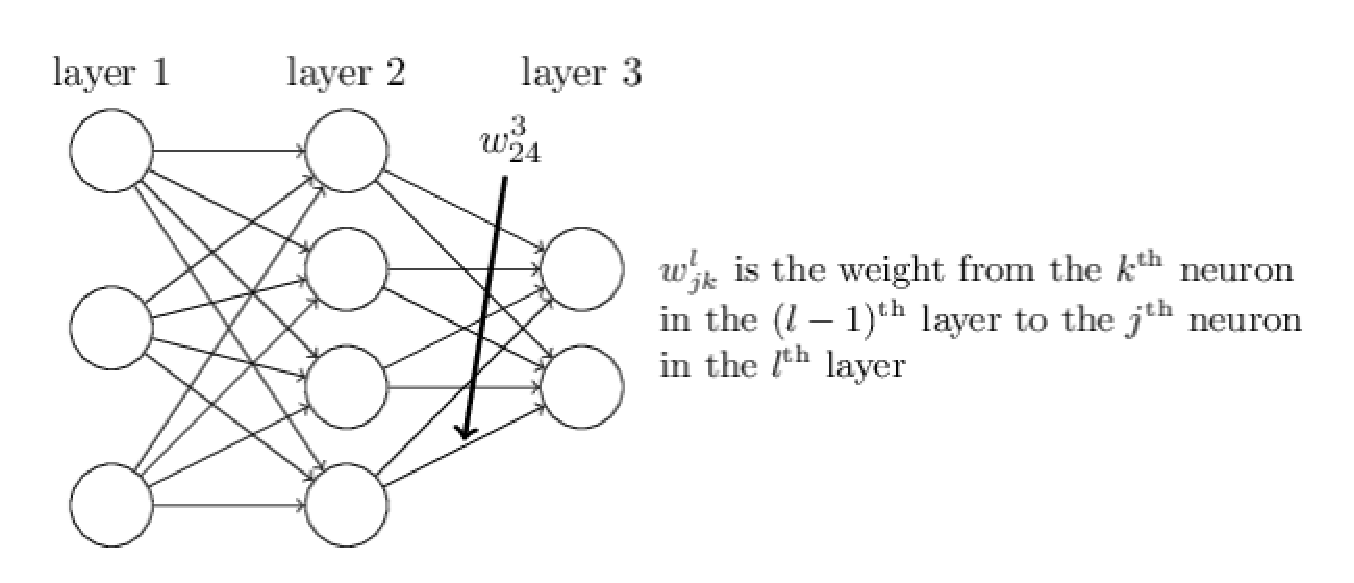
\includegraphics[scale=0.5]{fig/weight_definition.eps}

\centerline {$a^{l}_j = \sigma\left(\sum_k w^{l}_{jk} a^{l-­1}_k + b^l_j \right)$}
向量表示:\par
\centerline{$a^{l} =\sigma(w^l a^{l-­1}+b^l)$}
矩阵表示:
\begin{center}
$a^l = \sigma(z^l)$\\
$z^l \equiv w^l a^{l-­1}+b^l$
\end{center}
其中:\par
\centerline{$z^l_j = \sum_k w^l_{jk} a^{l­-1}_k+b^l_j$}

\section{cost function的两个假设}
后向传播的目的是得到代价函数$C$对于网络中任意权重$w$或偏差$b$的偏导数:\par
\centerline{$\frac {\partial C}{\partial w}$ 和 $\frac{\partial C}{\partial b}$}

二次代价函数的形式:\par
\centerline{$C=\frac{1}{2n}\sum_x \|y(x)-­a^L(x)\|^2$}\par
\noindent$n$为样本数;$y=y(x)$为$x$对应的期望输出;$L$为网络层数;
$a^L=a^L(x)$是输入为$x$时的网络激活输出向量。

关于代价函数,什么样的假设可以使得后向传播能够应用起来?\par
\textcolor{red}{第一个假设}是代价函数能够被写成基于每一个独立的训练样本$x$求代价函数$C_x$的平均值:
$C_x=\frac{1}{n}\sum_x C_x$。二次代价函数满足此条件,其中每一个样本的代价为:
$C_x = \frac{1}{2} \|y­-a^L\|^2$ \par
需要这个假设的原因是因为后向传播实际上让我们能够基于每一个样本计算偏导数
$\partial C_x / \partial w$ 和 $\partial C_x / \partial b$
我们然后在整个选练样本基础上经过平均而求出
$\partial C / \partial w$ 和 $\partial C / \partial b$。

\textcolor{red}{第二个}关于代价函数的假设是可以把它当作神经网路激活输出的一个函数,
$cost \ C = C(a^L)$
二次型代价函数满足这个假定,因为对于每一个样本$x$,代价函数可以写成:\par
\centerline{$C = \frac{1}{2} \|y-­a^L\|^2 = \frac{1}{2} \sum_j (y_j-a^L_j)^2$}

Hadamard乘积或Schur乘积,$\odot$,即逐元素相乘

\section{backpropagation背后的基础四等式}
引入中间变量$\delta^l_j$,为做网络中第$l^{\rm th}$层第$j^{\rm th}$神经元的误差:
$\delta^l_j \equiv \frac{\partial C}{\partial z^l_j}$

\subsection{输出层的误差等式:}
\begin{align} 
\delta^L_j = \frac{\partial C}{\partial a^L_j} \sigma'(z^L_j). \tag{BP1}
\end{align}\par
矩阵形式:
\begin{align}
\delta^L = \nabla_a C \odot \sigma'(z^L). \tag{BP1a}\
\end{align}

\subsection{误差$\delta^l$用下一层的误差$\delta^{l+1}$表示:}
\begin{align}
\delta^l = ((w^{l+1})^T \delta^{l+1}) \odot \sigma'(z^l), \tag{BP2}
\end{align}

\subsection{代价函数相对网络中任意偏置变化率的等式:}
\begin{align}
\frac{\partial C}{\partial b^l_j} = \delta^l_j. \tag{BP3}
\end{align}
误差$\delta^l_j$和变化率$\partial C / \partial b^l_j$精确相同,简短形式为:
\begin{align}
\frac{\partial C}{\partial b} = \delta,\tag{31}
\end{align}

\subsection{代价函数相对网络中任意权重变化率的等式:}
\begin{align}
\frac{\partial C}{\partial w^l_{jk}} = a^{l-­1}_k \delta^l_j. \tag{BP4}
\end{align}
改写为:
\begin{align}
\frac{\partial C}{\partial w} = a_{\rm in} \delta_{\rm out}, \tag{32}
\end{align}
可以看到,(BP4) 的结果就是小的激活神经元的权重会比较缓慢的学习。

%%%%%%%%%%%%%%%
\begin{framed}
summary: backpropagation 方程
\begin{align*}
\delta^L & = \nabla_a C \odot \sigma'(z^L). \tag{BP1} \\
\delta^l & = ((w^{l+1})^T \delta^{l+1}) \odot \sigma'(z^l), \tag{BP2} \\
\frac{\partial C}{\partial b^l_j} & = \delta^l_j. \tag{BP3} \\
\frac{\partial C}{\partial w^l_{jk}} & = a^{l-­1}_k \delta^l_j. \tag{BP4}
\end{align*}
矩阵形式:

(BP1)重写为
\begin{align}
\delta^L = \Sigma'(z^L) \nabla_a C,\tag{1}
\end{align}
其中,$\Sigma'(z^L)$是一个对角线元素为$\sigma'(z^L_j)$的方阵,且其非对角线元素都是零。
此矩阵与$\nabla_a C$进行传统的矩阵乘法

(BP2)重写为:
\begin{align}
\delta^l = \Sigma'(z^l) (w^{l+1})^T\delta^{l+1} \tag{2}
\end{align}

合并(1)和(2)可得:
\begin{align}
\delta^l = \Sigma'(z^l)(w^{l+1})^T \ldots 
\Sigma'(z^{L-­1}) (w^L)^T \Sigma'(z^L) \nabla_a C \tag{3}
\end{align}
\end{framed}

\section{The Backpropagation}
\begin{framed}
\textbf{1. Input $x$:} \par \indent \indent \indent 
Set the corresponding activation $a^{1}$ for the input layer.

\textbf{2. Feedforward:} \par \indent \indent \indent 
For each $l = 2, 3, \ldots, L$ compute \par
\centerline{$z^{l} = w^l a^{l-­1}+b^l$ and $a^{l} = \sigma(z^{l})$.}

\textbf{3. Output error $\delta^L$:} \par \indent \indent \indent 
Compute the vector 
\[ \delta^{L} = \nabla_a C \odot \sigma'(z^L) . \]

\textbf{4. Backpropagate the error:} \par \indent \indent \indent 
For each $l = L-1,L-­2,\ldots, 2$ \ compute 
\[ \delta^{l} = ((w^{l+1})^T \delta^{l+1}) \odot \sigma'(z^{l}).\] \par

\textbf{5. Output: The gradient of the cost function}\par 
\centerline{$\frac{\partial C}{\partial w^l_{jk}} = 
a^{l-­1}_k \delta^l_j$ and $\frac{\partial C}{\partial b^l_j} = \delta^l_j$.}
\end{framed}

单个样本训练过程:
\begin{framed}
1. 输入训练样本集合 

2. 对于每一个训练样本$x$: \par
\indent \indent 设置对应的输入激活 $a^{x,1}$执行以下步骤:\par
\indent \indent $\circ$向前:对于每一层$l = 2, 3, \ldots, L$,计算 \par
\centerline{$z^{x,l} =w^l a^{x,l-­1}+b^l$ 和 $a^{x,l} = \sigma(z^{x,l})$}
\indent \indent $\circ$输出层误差$\delta^{x,L}$:计算向量
\[ \delta^{x,L} = \nabla_a C_x \odot \sigma'(z^{x,L}).\] 
\indent \indent $\circ$后向传播误差:对于每一层$l = L-­1,L-­2,\ldots, 2$,计算
\[ \delta^{x,l} = ((w^{l+1})^T \delta^{x,l+1}) \odot \sigma'(z^{x,l}).\]

3. 梯度下降:按下面规则更新,\par
\begin{align}
w_k & \longrightarrow w'_k = w_k - \eta \frac{\partial C_x}{\partial w_k} \\
b_l & \longrightarrow b'_l = b_l - \eta \frac{\partial C_x}{\partial b_l}
\end{align}
即,对于每一层$l = L, L-­1, \ldots, 2$,更新为: \par
\begin{align}
w^l & \rightarrow w^l­ -\frac{\eta}{m} \sum_x\delta^{x,l} (a^{x,l-­1})^T,\\ 
b^l & \rightarrow b^l­ -\frac{\eta}{m} \sum_x \delta^{x,l}
\end{align}
\end{framed}
%\cite{hu_improved_2015}


\chapter{Transfer Learning}
\section{RKHS}\cite{RKHS}
In functional analysis (a branch of mathematics), a \textbf{reproducing kernel Hilbert space (RKHS)} is a Hilbert space of functions in which point evaluation is a continuous linear functional.\par
Roughly speaking, this means that if two functions $f$ and $g$ in the RKHS are close in norm, i.e., $\|f-g\|$ is small, then $f$ and $g$ are also pointwise close, i.e., $|f(x)-g(x)|$ is small for all $x$. The reverse need not be true. \par
Let $X$ be an arbitrary set and $H$ a Hilbert space of real-valued functions on $X$. The evaluation functional over the Hilbert space of functions $H$ is a linear functional that evaluates each function at a point $x$,
\[ L_x : f \mapsto f(x) \forall f \in H \]

We say that $H$ is a reproducing kernel Hilbert space if $L_x$ is continuous at any $f$ in $H$ or, equivalently, if for all $x$ in $X$, $L_x$ is a bounded operator on $H$ , i.e. there exists some $M > 0$ such that
\[ L_x [f]:= f(x)\leq M	\|f\|_H \forall f \in H \] 

\section{MMD}\cite{MMD}
define the maximum mean discrepancy (MMD) as:\par
$p$ and $q$ be distributions defined on a domain $X$ \par
obervations: $X:=\left\lbrace x_1,\dots,x_m \right\rbrace $,
$Y:=\left\lbrace y_1,\dots,y_n \right\rbrace $,drawn independently and identically distributed (i.i.d.) from
$p$ and $q$ respectively

\begin{align}
MMD[\mathcal{F},p,q] := \underset{f\in \mathcal{F}}{sup} \left( E_{x\sim p } [f(x)] - E_{y\sim p } [f(y)] \right) \\
MMD[\mathcal{F},X,Y] := \underset{f\in \mathcal{F}}{sup} \left( \frac{1}{m} \sum_{i=1}^m f(x_i) - \frac{1}{n} \sum_{i=1}^n f(y_i)\right) 
\end{align}

Since $E_p[f(x)=\left\langle \mu[p],f\right\rangle]$,we may rewrite\par
\[ MMD[\mathcal{F},p,q]=\underset{\|f\|_{\mathcal{H} \leq 1}}{sup} \left\langle \mu[p] - \mu[q],f\right\rangle = \|\mu[p] - \mu [q]\|_{\mathcal{H}}\]

using $\mu [X] := \frac{1}{m}\sum_{i=1}^m$ and $k(x,x')=\left\langle \phi(x),\phi(x') \right\rangle $
empirical estimate of MMD is :
\[ MMD[\mathcal{F},X,Y]=\left[ \frac{1}{m^2} \sum_{i,j=1}^m k(x_i,y_j) - \frac{2}{mn} \sum_{i,j=1}^{m,n} k(x_i,y_j) + \frac{1}{n^2} \sum_{i,j=1}^n k(y_i,y_j) \right]^{\frac{1}{2}} \]

\section{Deep Transfer Network}\cite{Deep Transfer Network}

Denote $X^s=[x^s_1,\dots,x^s_{n^s}] \in R^{d\times n^s}$ and 
$X^t=[x^t_1,\dots,x^t_{n^t}] \in R^{d \times n^t}$ as the data matrices of $D^s$ and $D^t$ respectively,$X=[X^s,X^t]$ as the combination of $X^s$ and $X^t$ \par
\begin{align}
MMD&=\|\frac{1}{n^s} \sum_{i=1}^{n^s}x_i^s - \frac{1}{n^t} \sum_{j=1}^{n^t}x_j^t \|^2_2\\
&=Tr(XMX^T)
\end{align}
where $M$ is the MMD matrix. Let $M_{ij}$ be one element of $M$.\par
\begin{align}
M_{ij}=\{
\end{align}
\include{chp/Whiten}
% 画网络图
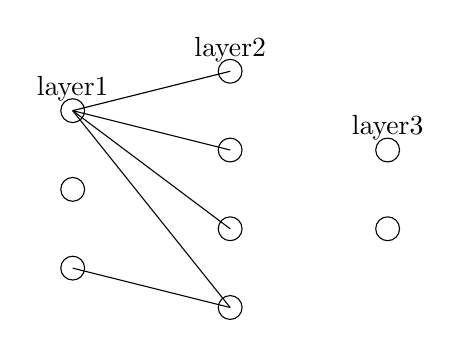
\begin{tikzpicture}
\coordinate (a1) at (0,0);
\coordinate (a2) at (0,-1);
\coordinate (a3) at (0,-2);
\coordinate (b1) at (2,0.5);
\coordinate (b2) at (2,-0.5);
\coordinate (b3) at (2,-1.5);
\coordinate (b4) at (2,-2.5);
\coordinate (c1) at (4,-0.5);
\coordinate (c2) at (4,-1.5);

\draw (a1) circle (1ex) node[above]{layer$1$};
\draw (a2) circle (1ex);
\draw (a3) circle (1ex);
\draw (b1) circle (1ex) node[above]{layer$2$};
\draw (b2) circle (1ex);
\draw (b3) circle (1ex);
\draw (b4) circle (1ex);
\draw (c1) circle (1ex) node[above]{layer$3$};
\draw (c2) circle (1ex);

\draw (a1) -> (b1); \draw (a1) -> (b2);\draw (a1) -> (b3);\draw (a1) -> (b4);
\draw (a3) -> (b4);
\end{tikzpicture}

\dots \ldots\\
inpuT. Yes\\
\phantom{4456}abcd\\
efg

\verb"*&^%$#\" \\
\verb)*&^%$#\)
\verb*)*&^% $# \*)

$\text{减数}-\text{被减数}=\text{差}$	% 网络图

%% 参考文献  %%%%%%%%%%%%%%%%%%%%%%%%%%%%%%%%%%%%%
%%%% bibtex方式 
\bibliographystyle{ieeetr}
\bibliography{mg_BibTex}

%% bibliography方式 
%\begin{thebibliography}{mg}
%\bibitem{positive definite  matrix} “Positive-definite matrix - Wikipedia, the free encyclopedia.” [Online]. Available: https://en.wikipedia.org/wiki/Positive-definite\_matrix. [Accessed: 09-Sep-2016].
%
%\bibitem{Hilbert space} “Hilbert space - Wikipedia, the free encyclopedia.” [Online]. Available: https://en.wikipedia.org/wiki/Hilbert\_space. [Accessed: 08-Sep-2016]. 
%\end{thebibliography}


%%%%%%%%%%%%%%%%%%%%%%%%%%%%%%%%%%%
\end{CJK}
\end{document}